\label{chapter:used-molecules}
The following molecules have been used to conduct experiments. Images show the molecules in a \SI{4x4}{\nano \meter} area in an orthographic projection. Since all of them feature distinct properties, all of them are introduced in the following subsections. We will utilize porphyrine derivatives (\autoref{sec:TBP}), functionalized pyrene molecules (\autoref{sec:pyrene}), helicene species (\autoref{sec:helicene}) and coronene (w\/o central borazine functionalization, see \autoref{sec:hbc}).

All the depicted molecules are modeled in Hyperchem\cite{_hyperchemtm_1111} and calculated for optimized geometry with the AM1+ method. Afterwards their positions are exported and remodeled in blender. Note that this does not change their geometry. It is only for better control of the output (faster and more accurate model building especially in 3D) and for some aesthetic reasons.

%%%%%%%%%%%%%%%%%%%%%%%%%%%%%%%%%%%%%%%%%%%%%%%%%%%%%%%%%%%%%%%%%%%%%%%%%%%%%%%%%%%%%%%%%%%
%%%%%%%%%%%%%%%%%%%%%%%%%%%%%%%%%%%	pyrenes   %%%%%%%%%%%%%%%%%%%%%%%%%%%%%%%%%%%%%%%%%
\subsection{Pyrene: Pyridilethynyl functionalized pyrenes}
\label{sec:pyrene}\index{molecules!Pyrene}
\begin{itemize}
	\item[tetra-pyrene:] 1,3,6,8-Tetra(4-Pyridylethynyl)pyrene
	\item[cis-pyrene:] 1,8-Bis(4-Pyridylethynyl)pyrene
	\item[trans-pyrene:] 1,6-Bis(4-Pyridylethynyl)pyrene
\end{itemize}

\begin{figure}[]
	\begin{center}
		\subfigure[Tetra-configuration]{
			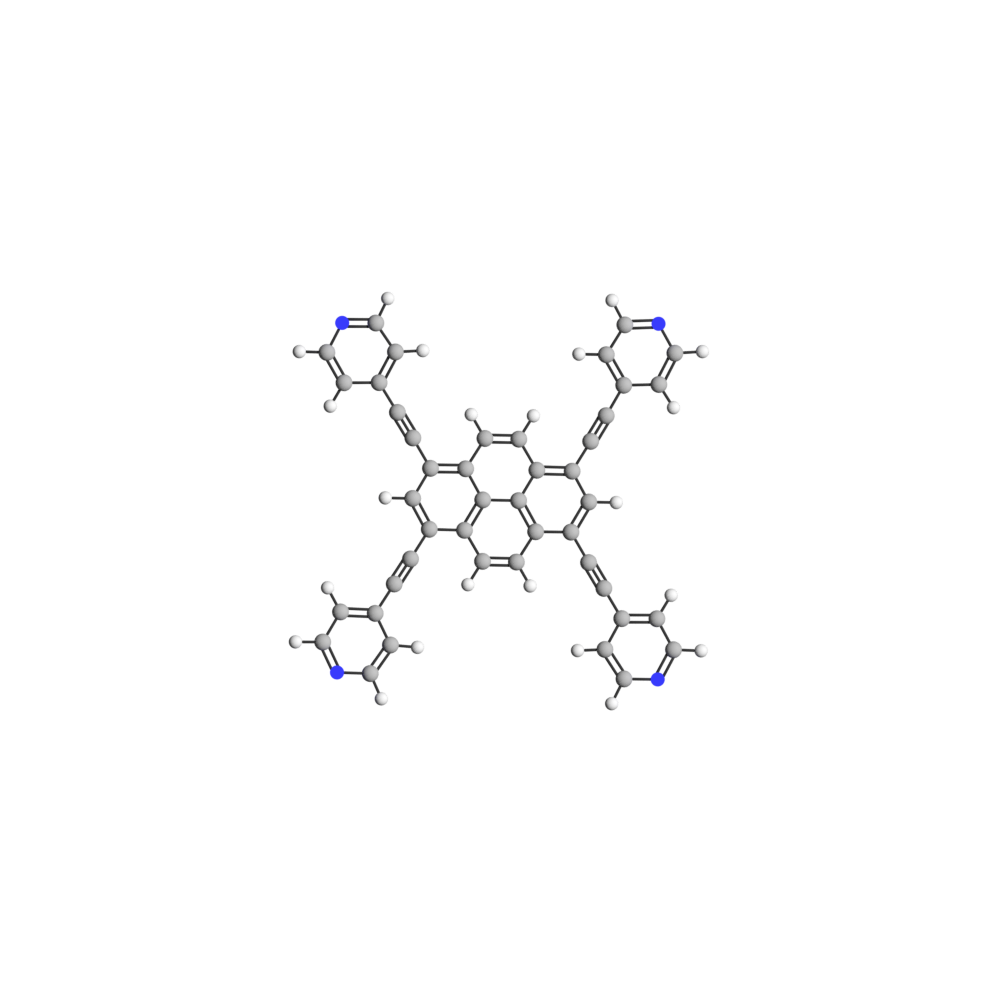
\includegraphics[width=0.3\textwidth]{./images/molecules/pyrene-tetra}
			\label{fig:pyrene-tetra}
		} 
		\subfigure[Trans-configuration]{
			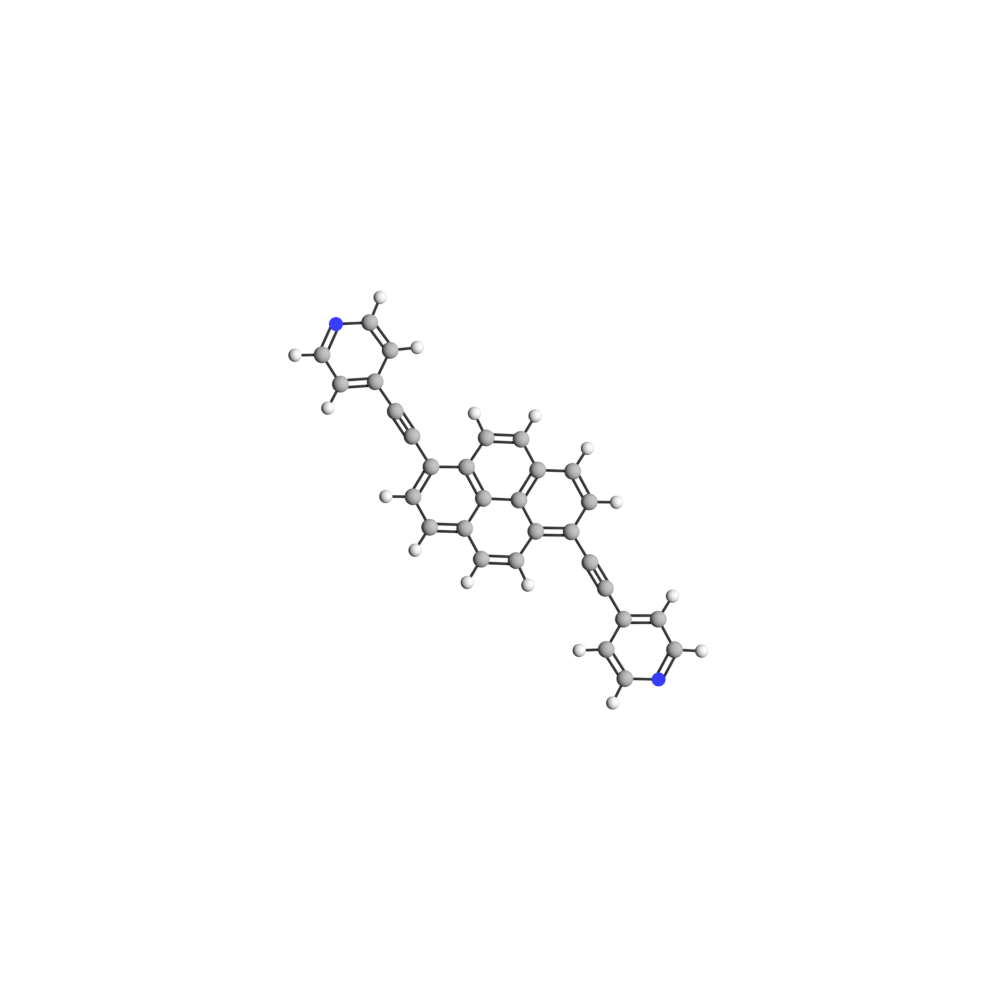
\includegraphics[width=0.3\textwidth]{./images/molecules/pyrene-trans}
			\label{fig:pyrene-trans}
		} 
		\subfigure[Cis-configuration]{
			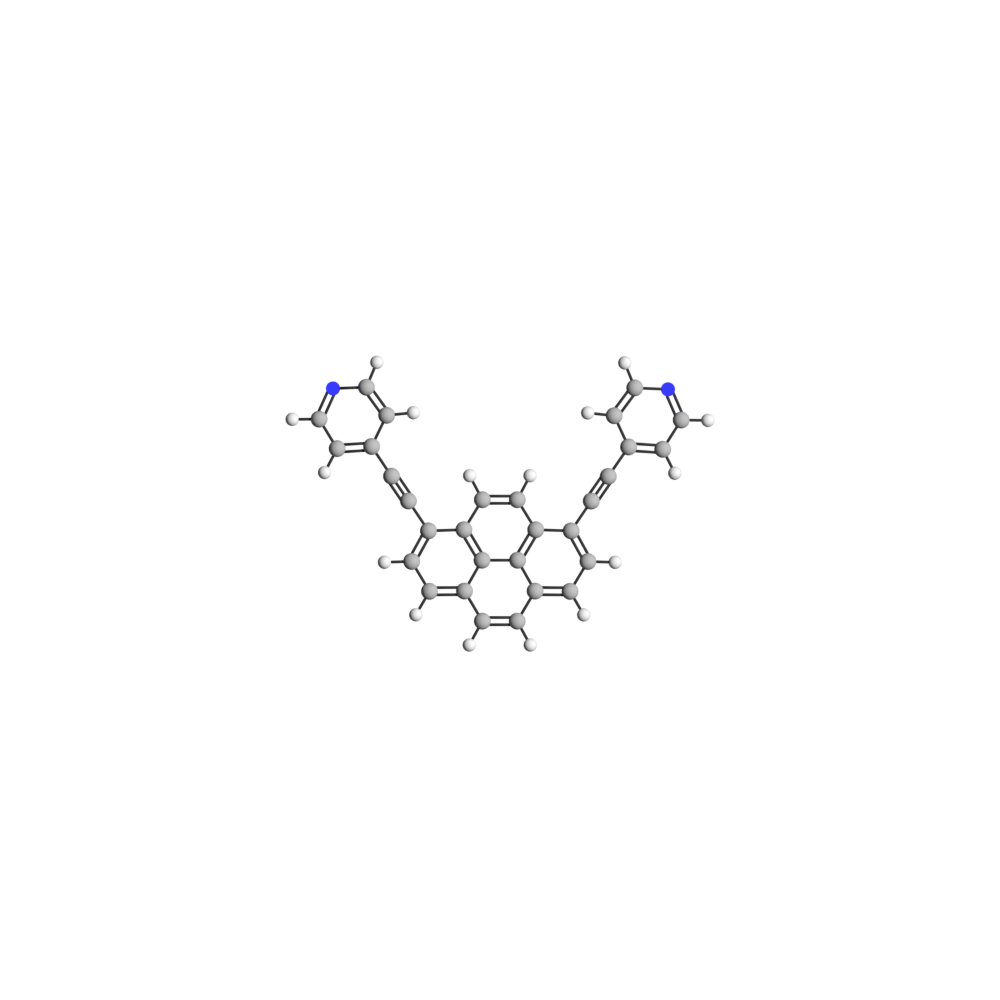
\includegraphics[width=0.3\textwidth]{./images/molecules/pyrene-cis}
			\label{fig:pyrene-cis}
		}
	\end{center}
	\caption{Pyridyl-Pyrene molecules in trans- \subref{fig:pyrene-trans} and cis- \subref{fig:pyrene-cis} and tetra- \subref{fig:pyrene-tetra} configuration}
	\label{fig:pyrene}
\end{figure}

Pyrene molecules, first investigated in 1973 \cite{khan_electronic_1973}, are 4 ortho-fused carbon rings to result in a rhombic structure. As many other $\pi$ conjugated systems they show interesting optoelectronic properties like \cite{crawford_experimental_2011, lee_enhanced_2012, feng_functionalization_2016, kurata_diarylamino-_2017, maeda_alkynylpyrenes_2006, kurata_diarylamino-_2017} and assembly was investigated \cite{pham_self-assembly_2014, matena_aggregation_2010, della_pia_anomalous_2014, pham_comparing_2016}. Here they are used to investigate the influence of the number and position of functional groups on these properties. The very same species have been investigated on Cu(111) albeit data adsorbed on \textit{h}-BN/Cu(111) was lacking up to this point. The nano-pattering effect of the \textit{h}-BN substrate is used here to modulate the wide band gap of the species and therefor their optical properties.
%%%%%%%%%%%%%%%%%%%%%%%%%%%%%%%%%%%%%%%%%%%%%%%%%%%%%%%%%%%%%%%%%%%%%%%%%%%%%%%%%%%%%%%%%%%
%%%%%%%%%%%%%%%%%%%%%%%%%%%%%%%%%%%	HBBNC + HBC   %%%%%%%%%%%%%%%%%%%%%%%%%%%%%%%%%%%%%%%%%
\subsection{Coronene: HBBNC and HBC}
\label{sec:hbc}\index{molecules!Coronene}
\begin{itemize}
	\item[HBBNC:] 2-8-14-trixylyl-hexaphenyl borazinocoronene
	\item[HBC:] 2,8,14-trixylyl-hexabenzocoronene	
\end{itemize}

\begin{figure}[]\centering
	\subfigure[HBBNC]{
		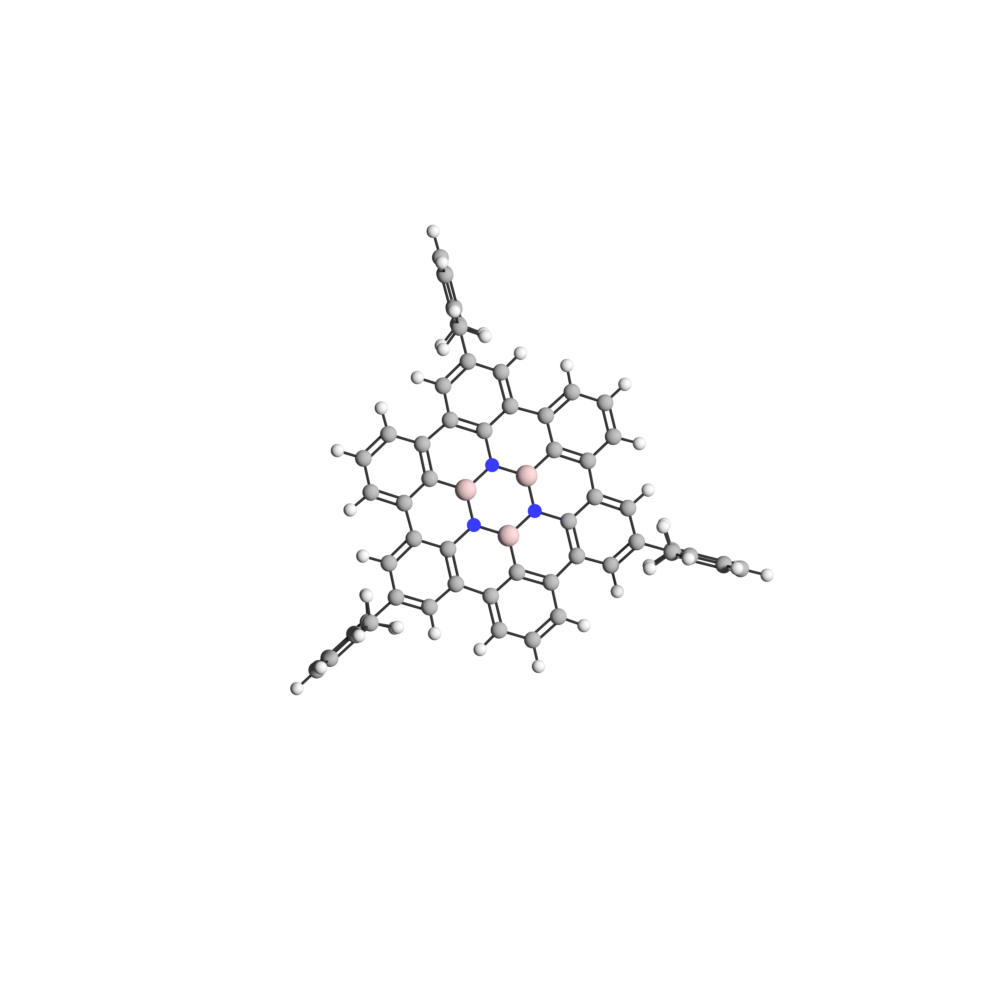
\includegraphics[width=0.3\textwidth]{./images/molecules/HBBNC}
		\label{fig:HBBNC}
	} \quad
	\subfigure[HBC]{
		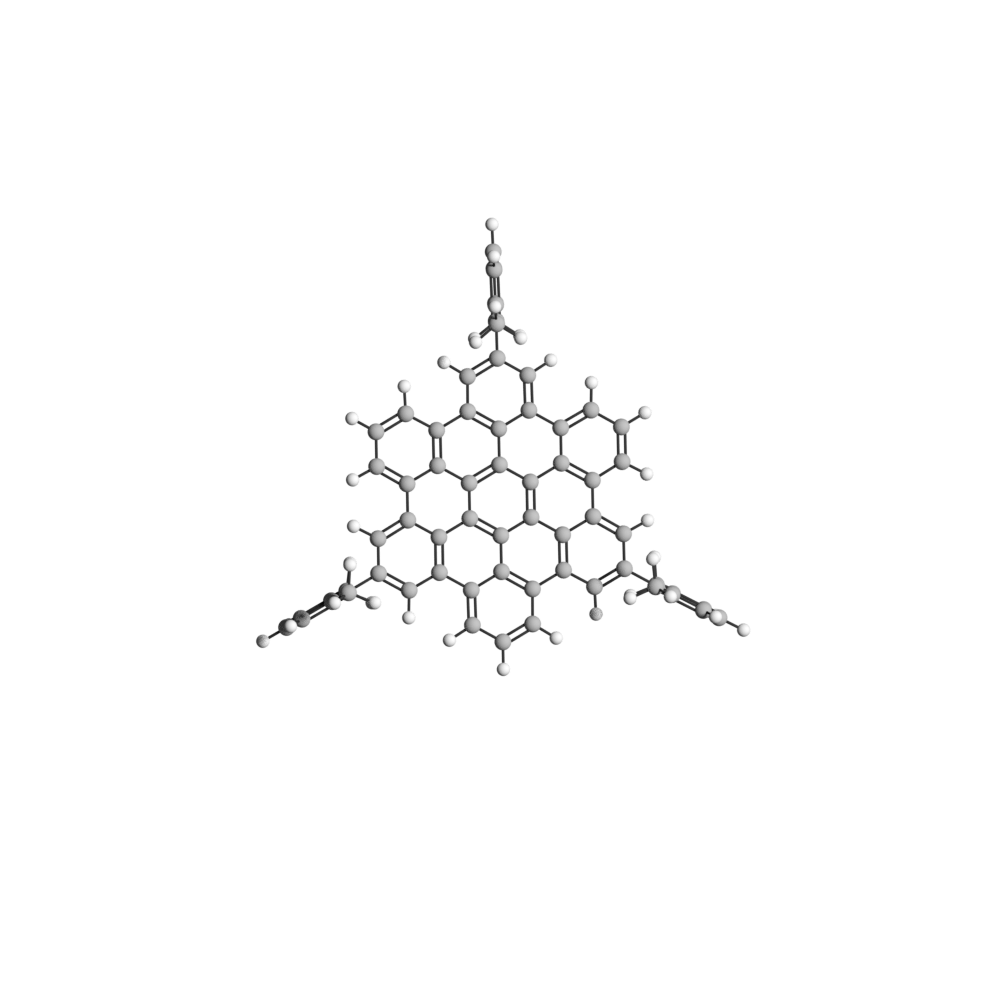
\includegraphics[width=0.3\textwidth]{./images/molecules/HBC}
		\label{fig:HBC}
	} \quad
	\caption{\subref{fig:HBBNC} HBBNC and \subref{fig:HBC} HBC}
	\label{fig:HBBNC+HBC}
\end{figure}

While in 2015\cite{Krieg_construction_2015} and 2016 \cite{Ciccullo_Quasi-Free-Standing_2016} hexy-peri-Hexabenzoborazino coronene (HBBNC) was synthesized, its bad solubility prohibited experiments. In 2017 the synthesis \cite{dosso_synthesis_2017} of a soluble, BN-doped coronene derivative by substitution of the central carbon ring was successful. By using HBBNC the HOMO-LUMO band gap could be widened and shows blue-shifted emission properties\cite{dosso_synthesis_2017} compared to its all-carbon counterpart. Investigations with STM are performed on Au(111) \cite{Krieg_construction_2015}.
Here the central $(BN)_3$ core is oriented to point all nitrogen atoms towards the leg functionalization.
Due to the different electro negativity of the atomic species adsorption of gases in the central part can be interesting effects to look out for. In this thesis we focused on the geometric properties of this molecule first. Please refer to \autoref{section:HBBNC} for detailed information.


%%%%%%%%%%%%%%%%%%%%%%%%%%%%%%%%%%%%%%%%%%%%%%%%%%%%%%%%%%%%%%%%%%%%%%%%%%%%%%%%%%%%%%%%%%%
%%%%%%%%%%%%%%%%%%%%%%%%%%%%%%%%%%%	TPCN      %%%%%%%%%%%%%%%%%%%%%%%%%%%%%%%%%%%%%%%%%
%\subsection{TPCN}
%TPCN can be evaporated with an OMBE. Temperatures used are typically \SI{490}{\celsius}, evaporation time depends on the intended coverage. 
%\begin{itemize}
%	\item [TPCN:] Tetra[(4-cyanophenyl)-phen-4-yl] porphyrin has four arms attached to the meso-positions of the macrocycle. Each is build up from two chained phenyl rings with one end attached to the macrocycle and the other one attached to a C-N end group. Due to their flexibility, they are versatile connection segments \cite{fendt_modification_2009}.
%\end{itemize}
%
%\begin{figure}[]
%	\centering
%	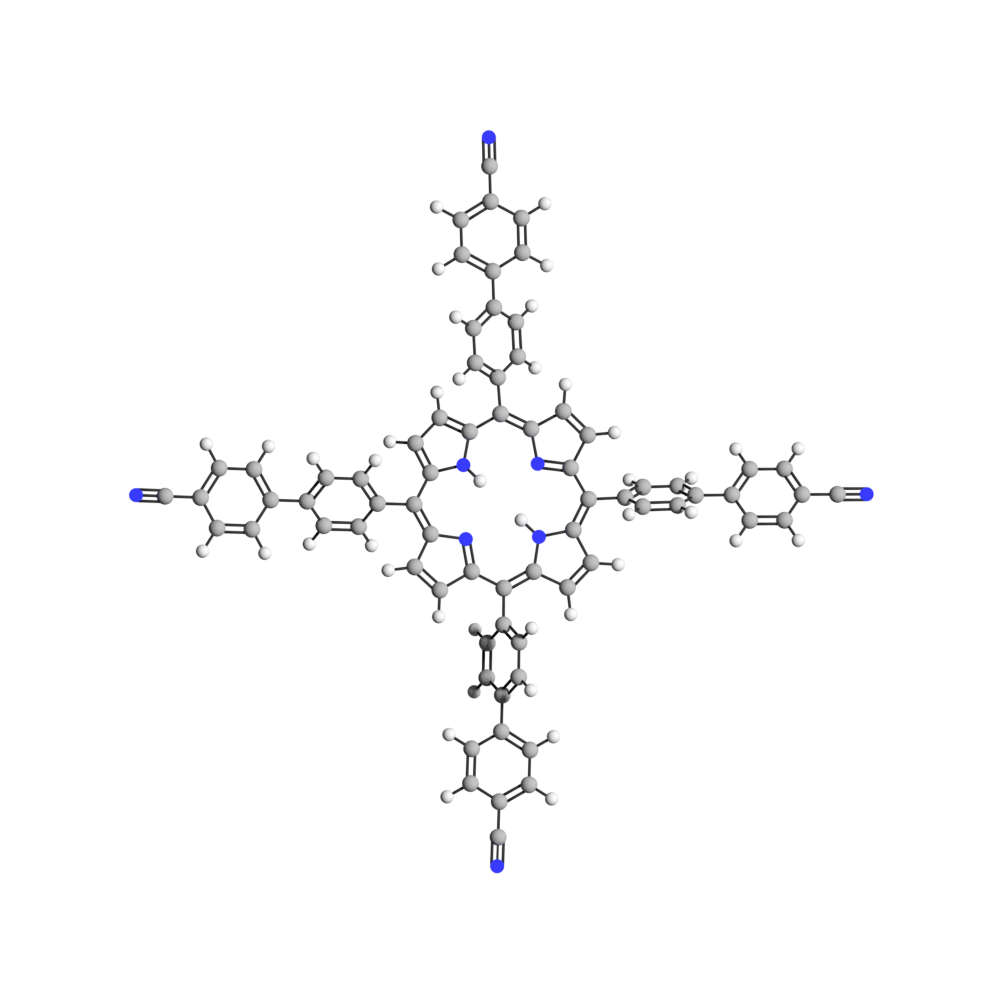
\includegraphics[width=0.3\textwidth]{./images/molecules/TPCN}
%	\caption{TPCN molecule}
%	\label{fig:TPCN}
%\end{figure}


%%%%%%%%%%%%%%%%%%%%%%%%%%%%%%%%%%%%%%%%%%%%%%%%%%%%%%%%%%%%%%%%%%%%%%%%%%%%%%%%%%%%%%%%%%%
%%%%%%%%%%%%%%%%%%%%%%%%%%%%%%%%%%%nitro-prophines%%%%%%%%%%%%%%%%%%%%%%%%%%%%%%%%%%%%%%%%%
\subsection{Porphine: [di-[tert-butyl]-phenyl)]-porphyrin derivatives}
\label{sec:TBP}\index{molecules!TBP}
Tetrapyrroles like porphyrins and phthalocyanines play important roles in biological systems \cite{battersby_tetrapyrroles_2000}. Both species are able to incorporate metal atoms that control the function. Not only are they interesting model systems to study interaction towards a (metallic) substrate\cite{auwarter_porphyrins_2015, auwarter_controlled_2007, diller_vacuo_2016}. Their use in metal-organic frameworks highlights the use of scientific knowledge to design "real world" sensor applications\cite{Lustig_Metal-organic_2017}. 


Tert-butyl functionals have been used in a variety of molecules \cite{moresco_conformational_2001}. Due to their bulky nature, they electronically decouple the porphyrin’s de-localized p-orbital system from the metallic surface just by lifting the molecule. They may undergo heavy conformational deformation when outer influences (like metalization of the central porphine core) act on the molecule \cite{stark_massive_2014}. Switching capabilities are well investigated \cite{loppacher_direct_2003} and it is possible to switch them with the STM tip \cite{ditze_energetics_2014}. Experiments with similar molecules investigate the heat-induced formation of 1D and 2D conglomerates on a Au(111) surface.\cite{pham_heat-induced_2015}

\begin{itemize}
	\item Free base nitrophenyl - 5,10,15 Tri [di-[tert-butyl]-phenyl)]-porphyrin \index{nitro porphin} has 3(2) di-tert-butyl-phenyl groups attached to the porphine macro cycle at the meso-positions of the molecule. The free meso-positions are occupied with nitrophenyl groups as shown in \autoref{fig:TBP-single} If more than one functional group is present, one can distinguish between trans (\autoref{fig:TBP-trans}) and cis configuration (\autoref{fig:TBP-cis}), whether the two functional groups are opposite or neighboring.
	\item The appearance of STM data is correlated to the molecular configuration according to \cite{mishra_current-driven_2015} meaning that the lobes consisting of (3,5-di-tert-butylphenyl) are imaged as bright protrusions, while the functional nitro group is imaged fainter. This holds true for cis- and trans-substituted molecules\cite{yokoyama_selective_2001}.
	\item Tert-butyl groups can rotate and form flexible legs. Interaction with the substrate results in adsorption-induced conformational changes.\cite{ecija_dynamics_2016}
\end{itemize}
Drawings for various functional groups and molecules can be found in \cite{jorgensen_salem_1973}

\begin{itemize}
	\item[one-leg:]  	 5,10,15-Tri(3,5-di-tert-butylphenyl)-   20-(Nitrophenyl)porphyrine
	\item[two-leg cis:] 	5,10-Bis(3,5-di-tert-butylphenyl)-15,20-Bis(Nitrophenyl)porphyrine
	\item[two-leg trans:] 	5,15-Bis(3,5-di-tert-butylphenyl)-10,20-Bis(Nitrophenyl)porphyrine
\end{itemize}

\begin{figure}[]\centering
	\subfigure[Single functional group]{
		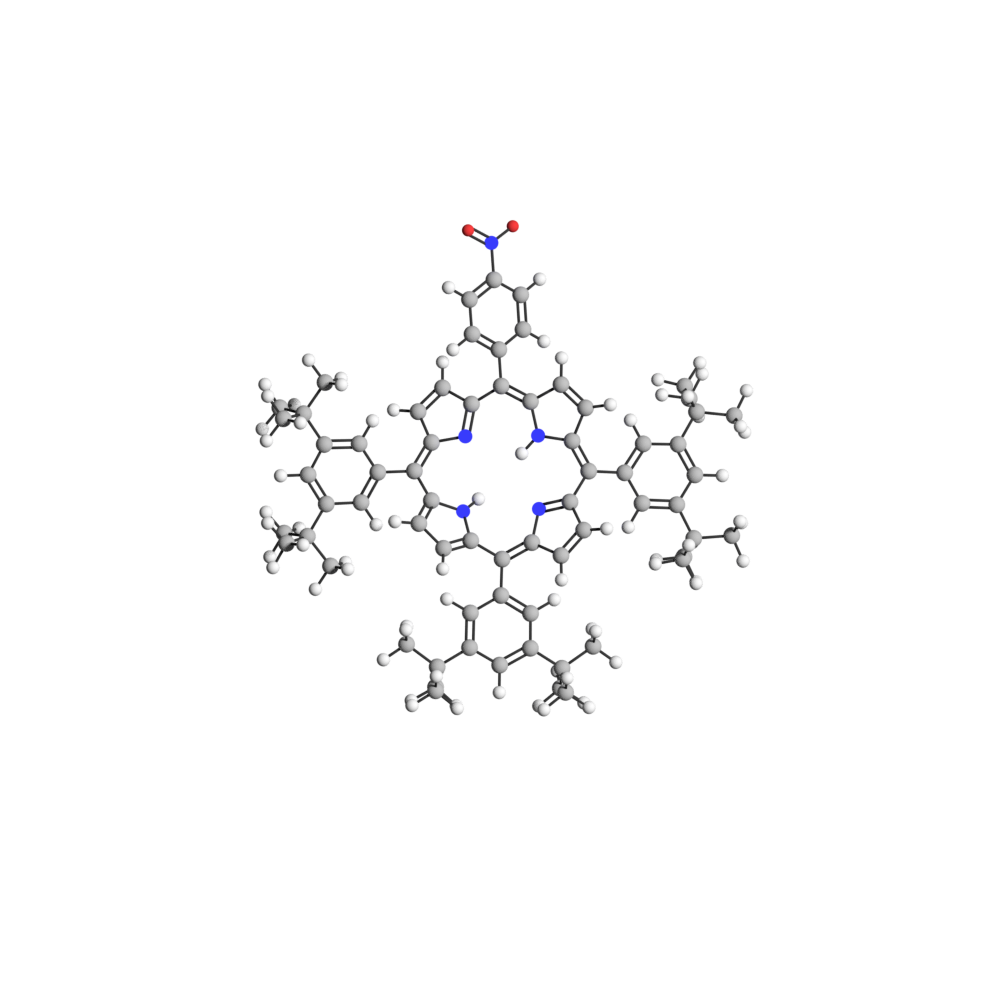
\includegraphics[angle=90, width=0.3\textwidth]{./images/molecules/TBP-single}
		\label{fig:TBP-single}
	} %
	\subfigure[Trans-configuration]{
		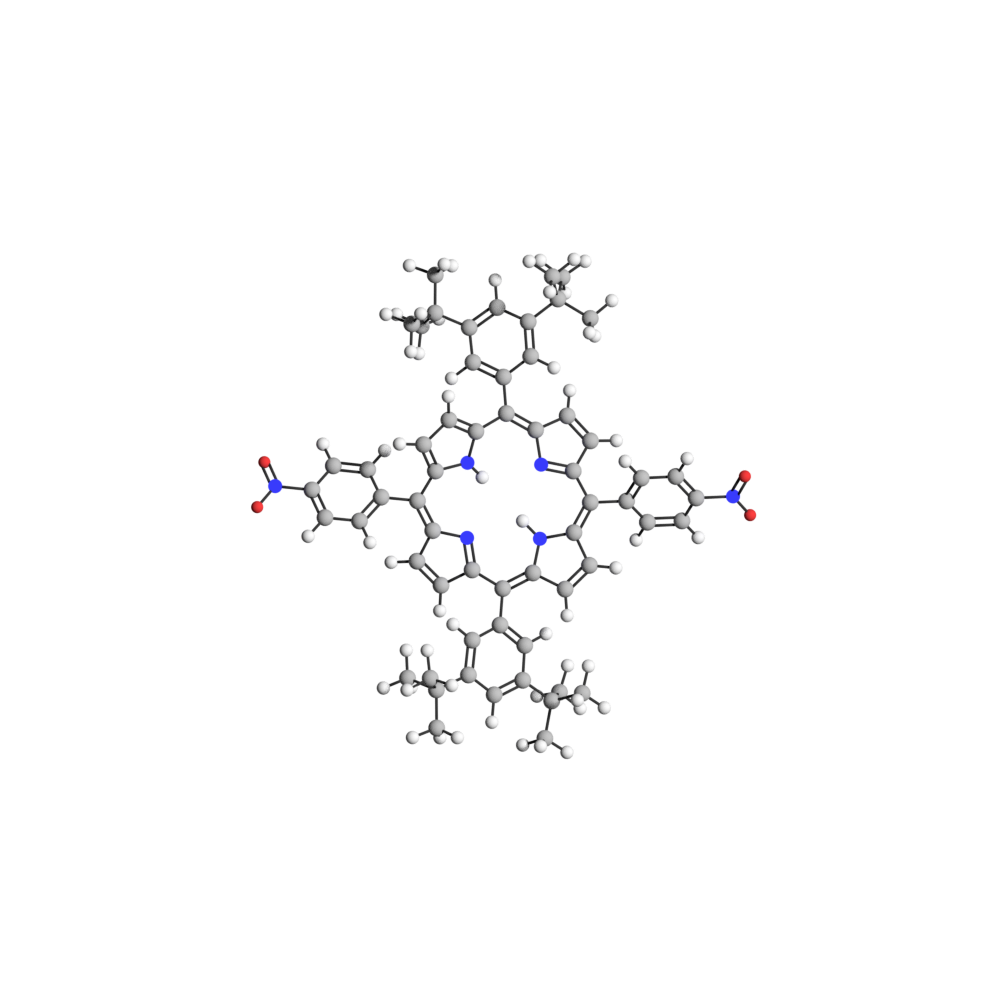
\includegraphics[angle=0, width=0.3\textwidth]{./images/molecules/TBP-trans}
		\label{fig:TBP-trans}
	} %
	\subfigure[Cis-configuration]{
		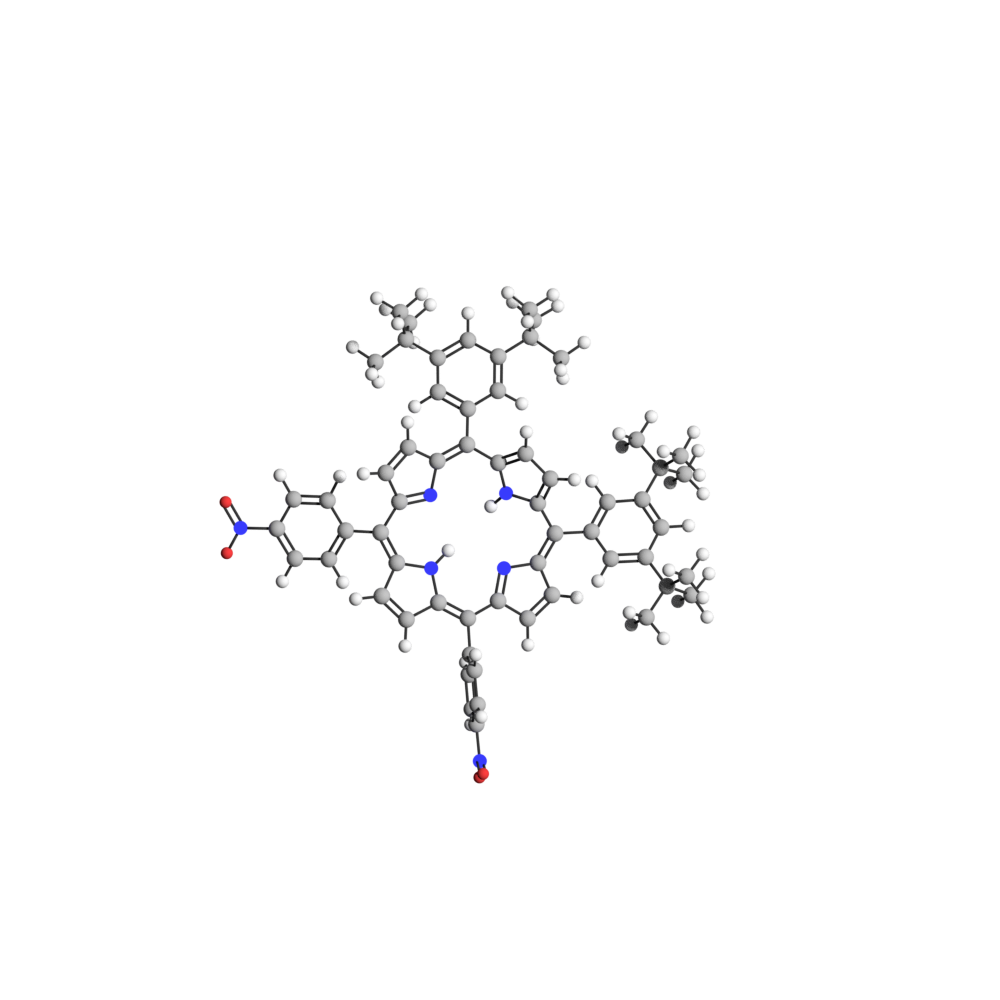
\includegraphics[angle=0, width=0.3\textwidth]{./images/molecules/TBP-cis}
		\label{fig:TBP-cis}
	} %
	\caption{Functionalized tert-butyl-phenyl-porphines. \subref{fig:TBP-single} shows a single functionalized porphine molecules. An additional function may be added in \subref{fig:TBP-cis} cis-  and \subref{fig:TBP-trans} position.}
	\label{fig:TBP}
\end{figure}	
	%%%%%%%%%%%%%%%%%%%%%%%%%%%%%%%%%%%%%%%%%%%%%%%%%%%%%%%%%%%%%%%%%%%%%%%%%%%%%%%%%%%%%%%%%%%
	%%%%%%%%%%%%%%%%%%%%%%%%%%%%%%%%%%%	helicenes %%%%%%%%%%%%%%%%%%%%%%%%%%%%%%%%%%%%%%%%%
	\subsection{Helicene: Cyano functionalization of helicenes}
	\label{sec:helicene}\index{molecules!Helicene}
	\begin{itemize}
		\item[Dicyano-dibenzo-[5]helicene]: 7,8-Bis(cyano)-Dibenzo-helicene
	\end{itemize}
	
	\begin{figure}[]
		\centering
		\subfigure[Top view]{
			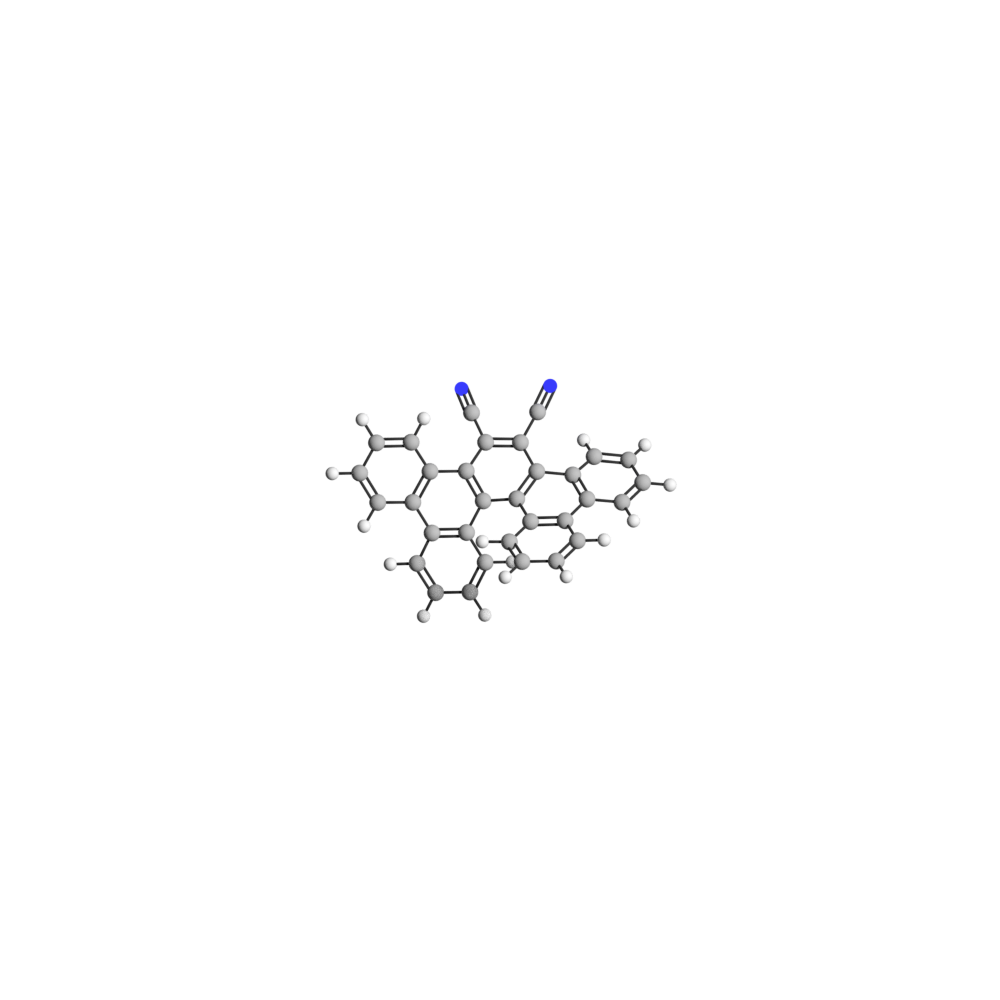
\includegraphics[width=0.3\textwidth]{./images/molecules/helicene}
			\label{fig:helicene-top}
		} \quad
		\subfigure[Side view]{
			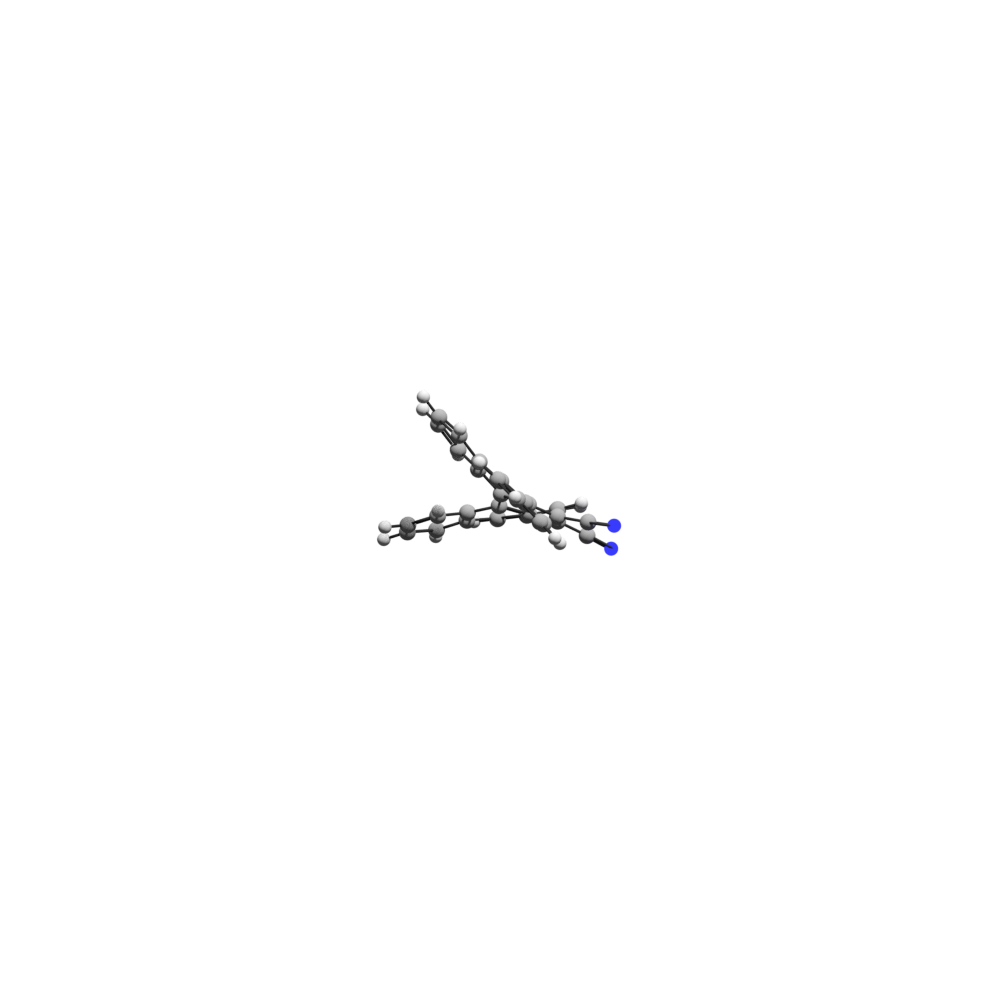
\includegraphics[width=0.3\textwidth]{./images/molecules/helicene-side}
			\label{fig:helicene-side}
		} \quad
		\caption{DCDB on copper surface. \subref{fig:helicene-top} Top view, \subref{fig:helicene-side} side view}
		\label{fig:helicene}
	\end{figure}
	
	Helicenes were first synthezised 1950's \cite{newman_synthesis_1956}. They consist of ortho condensed carbon rings that form a spiral due to overcrowding in their center. While they first drew attention due to their fluorescence properties \cite{vander_donckt_fluorescence_1968}, helicenes are interesting molecules because of their chiral feature. Two different turn directions exist, left and right. The molecules investigated in this work are fcuntionalized with two benzene rings at positions \underline{\qquad} and two cyano groups at positions seven and eight. For more information, please refer to \autoref{section:helicene}.